% arara: lualatex
\documentclass{beamer}
\AtBeginSection{\frame{\sectionpage}}

\defbeamertemplate{section page}{mine}[1][]{%
  \begin{centering}
    {\usebeamerfont{section name}\usebeamercolor[fg]{section name}#1}
    \vskip1em\par
    \begin{beamercolorbox}[sep=12pt,center]{part title}
      \usebeamerfont{section title}\insertsection\par
    \end{beamercolorbox}
  \end{centering}
}
\setbeamertemplate{section page}[mine]

\usepackage{pgfplots}

\title{High Pressure Ignition Chemistry of Alternative Fuels}
\author{Bryan W. Weber}
\institute{Prepared for Ph.D. Defense}
\date{June 19, 2014}

\beamertemplatenavigationsymbolsempty

\setbeamertemplate{footline}
{%
\begin{beamercolorbox}[sep=2mm]{}

\includegraphics[height=0.25in]{logo}
\hfill
{\color{gray} \insertpagenumber{}/\insertpresentationendpage}
\end{beamercolorbox}
}%

\graphicspath{ {figures/} }

\begin{document}

\maketitle

\begin{frame}{We use a lot of fuels to power the world}
    \only<1,3>{
    \begin{center}
        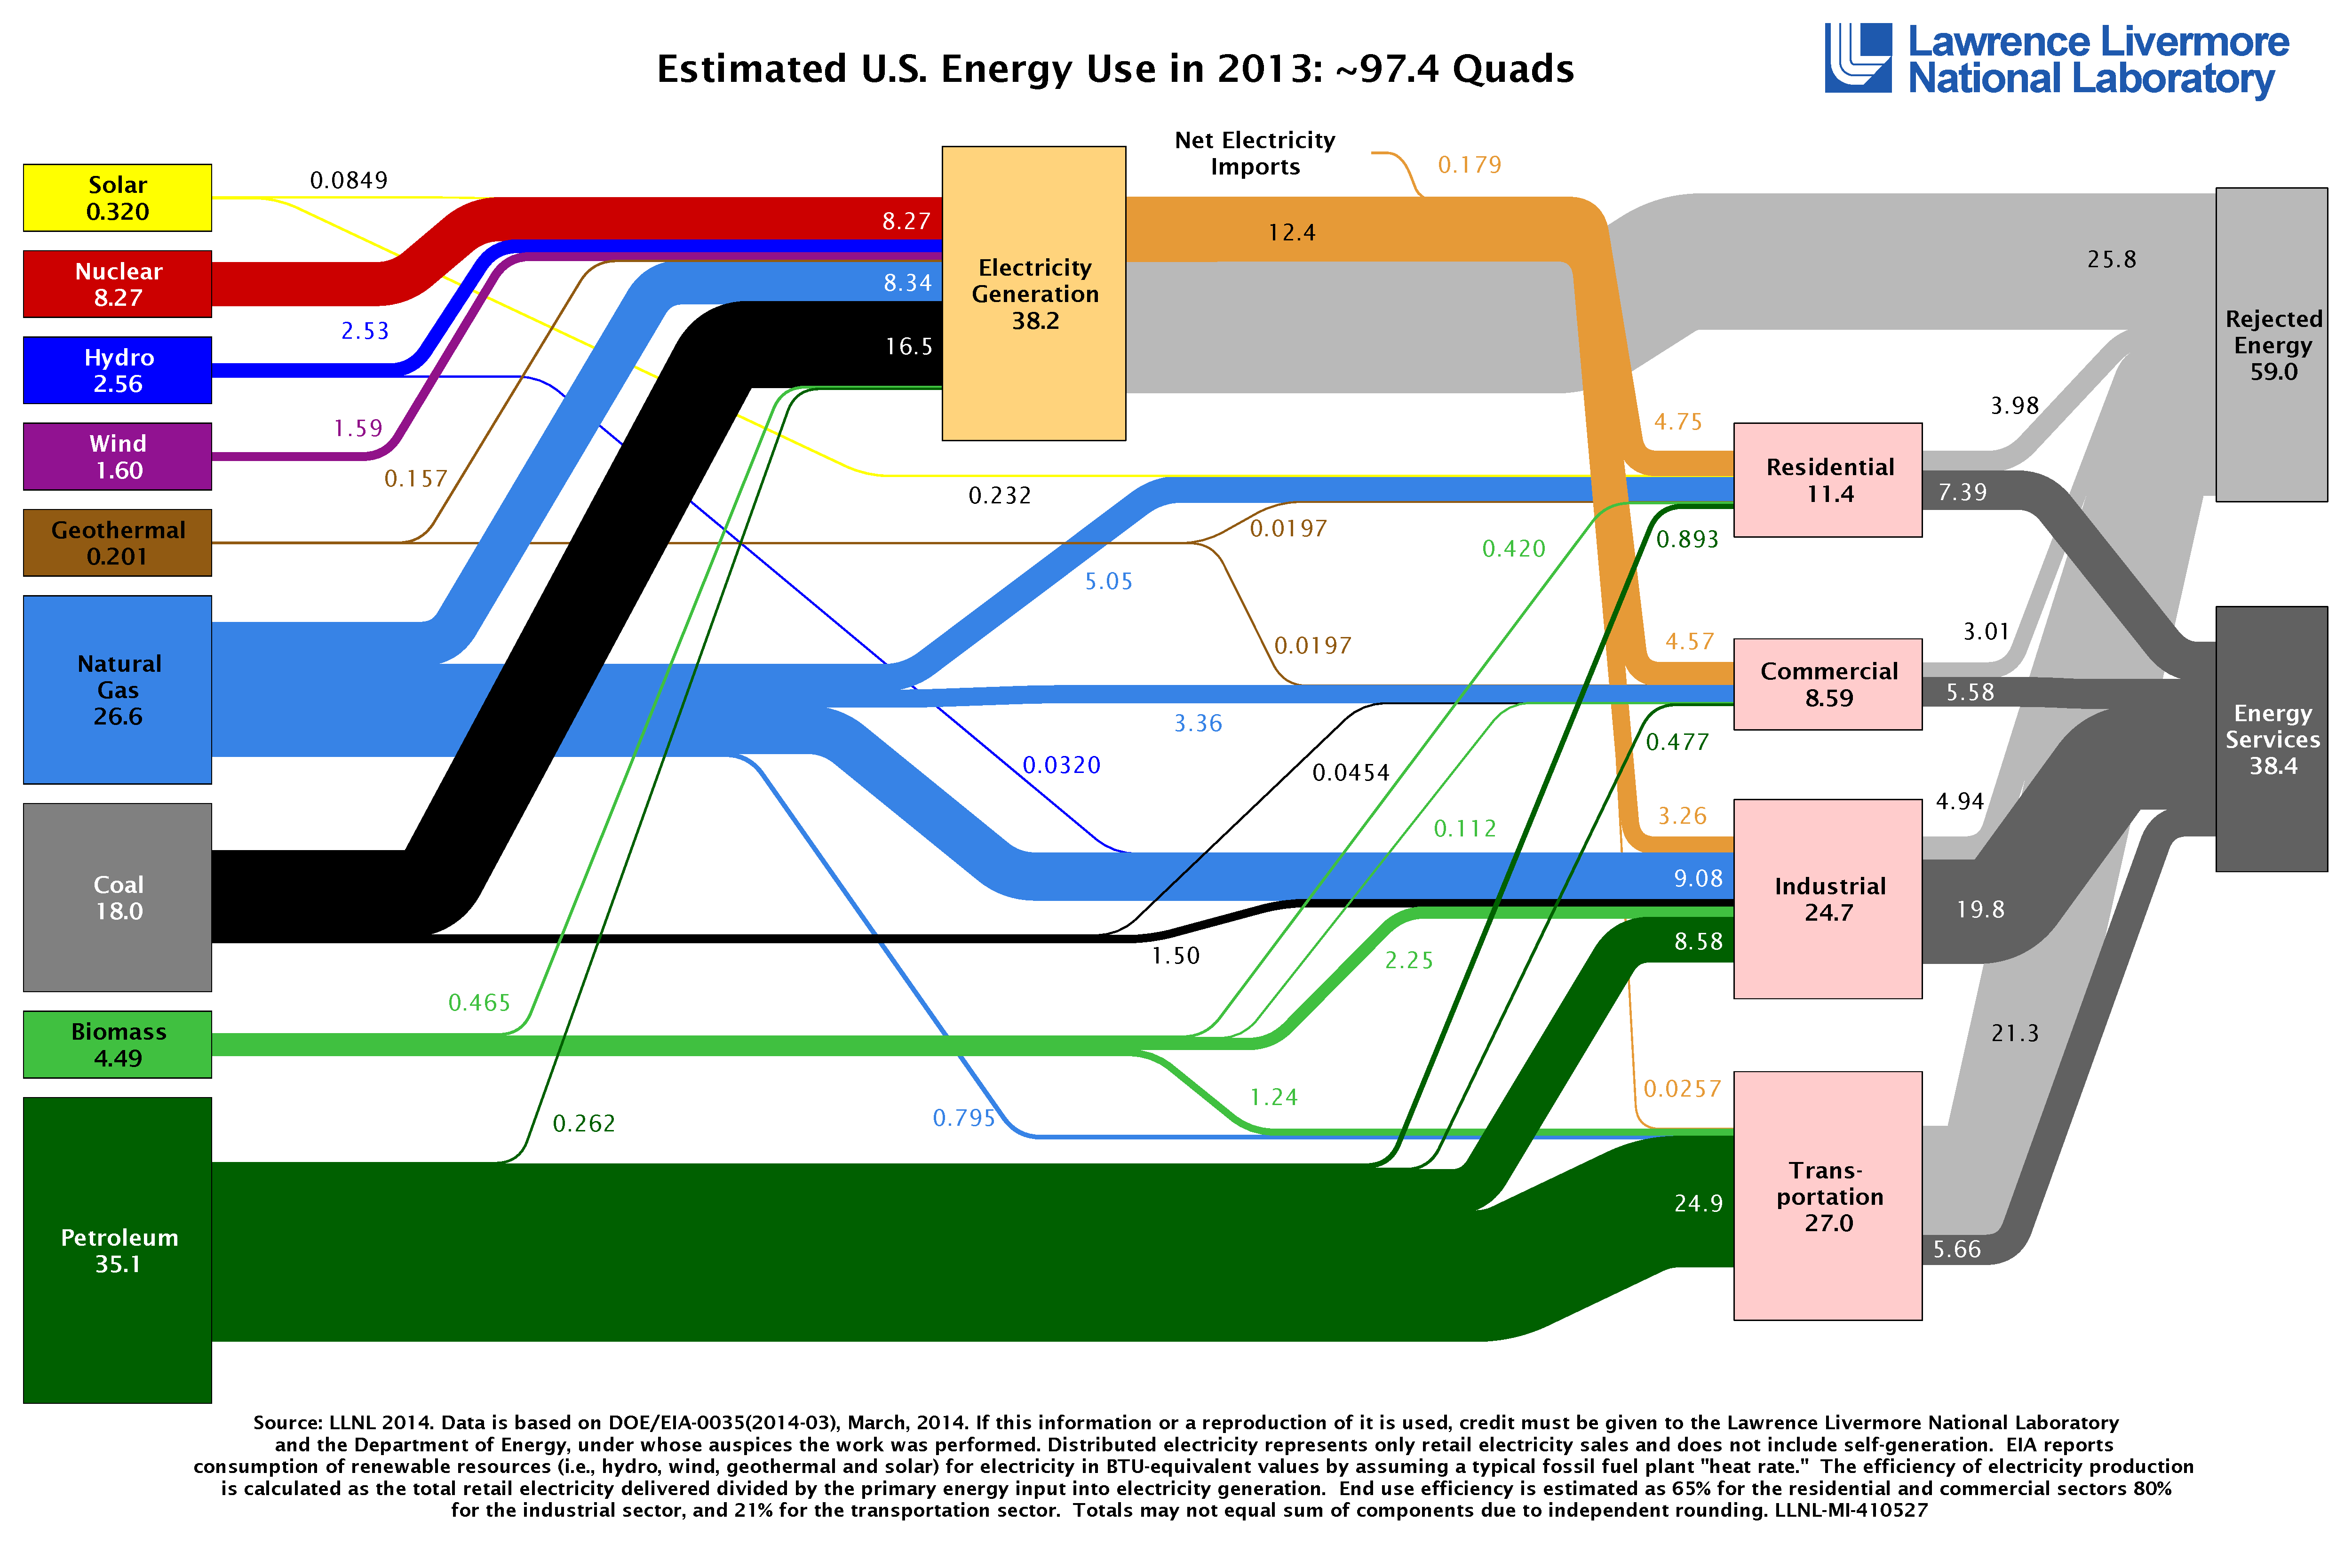
\includegraphics[width=\textwidth]{2013USEnergy}
    \end{center}
    }
    \only<2>{Could drive to the moon and back over 180 million times in a Telsa Model S with the amount of energy we use annually}
    % \begin{center}
        % \includegraphics[width=\textwidth]{me-to-moon}
    % \end{center}
    \only<4>{
    \begin{itemize}
        \item Combustion is predicted to remain the dominant energy conversion process for many years into the future
        \item The combustion of fossil fuels has been implicated in a number of harmful effects on human health, the environment, and the economy
        \item Two solutions have been proposed:
            \begin{itemize}
                \item Better engines
                \item Better fuels
            \end{itemize}
    \end{itemize}
    }
\end{frame}

\begin{frame}{Better engines have higher efficiency and lower emissions}
John Dec image
\end{frame}

\begin{frame}{Better fuels reduce emissions and eliminate dependence on fossil fuels}
    \begin{center}
        % 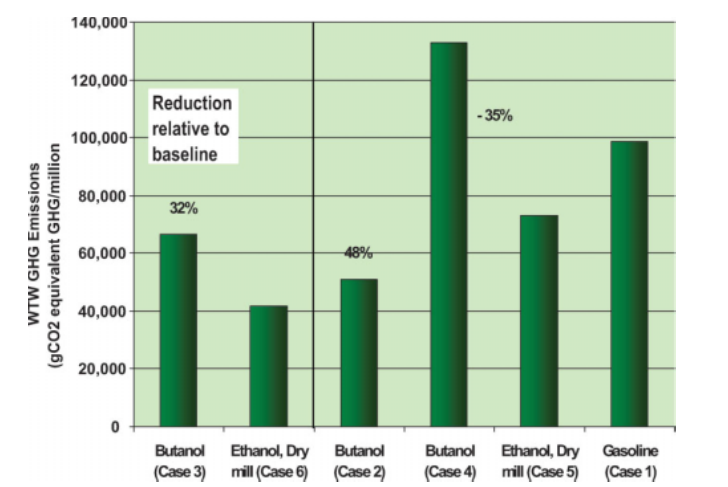
\includegraphics[width=\textwidth,height=0.85\textheight,keepaspectratio]{butanol-benefits}
        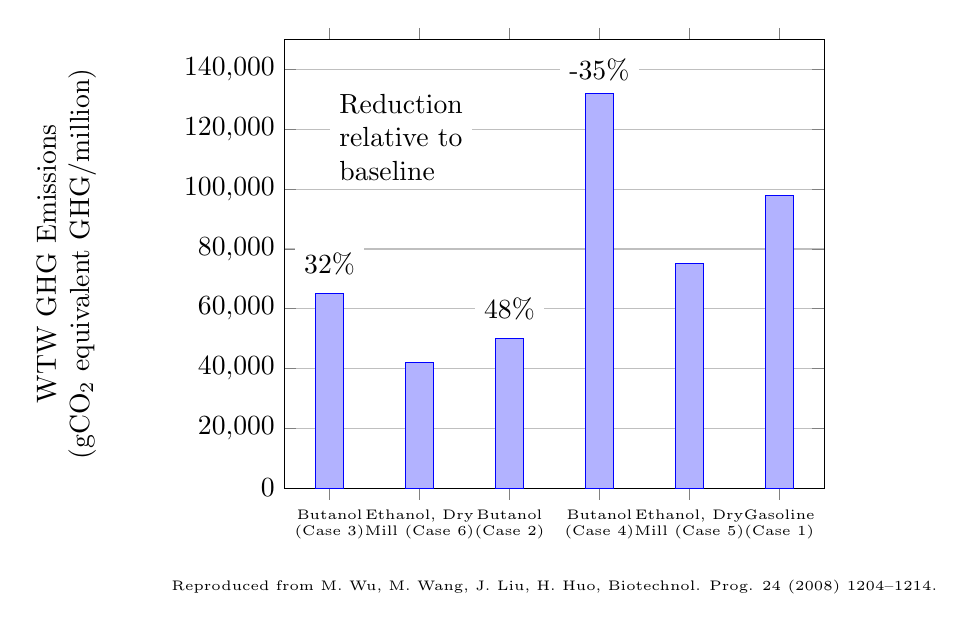
\begin{tikzpicture}
        \begin{axis}[
            ybar,
            scaled y ticks=false,
            ymin=0,ymax=150000,
            ytick={0,20000,40000,60000,80000,100000,120000,140000},
            yticklabel style={/pgf/number format/fixed},
            xtick={1,2,3,4,5,6},
            xticklabels={{Butanol\\(Case 3)}, {Ethanol, Dry\\Mill (Case 6)}, {Butanol\\(Case 2)}, {Butanol\\(Case 4)}, {Ethanol, Dry\\Mill (Case 5)}, {Gasoline\\(Case 1)}},
            xticklabel style={align=center,font=\tiny},
            ymajorgrids,
            ylabel={WTW GHG Emissions\\(gCO$_2$ equivalent GHG/million)},
            ylabel style={align=center,yshift=25pt},
            xlabel={Reproduced from M. Wu, M. Wang, J. Liu, H. Huo, Biotechnol. Prog. 24 (2008) 1204--1214.},
            xlabel style={font=\tiny,yshift=-8pt},
        ]
        \addplot coordinates {(1,65000) (2,42000) (3,50000) (4,132000) (5,75000) (6,98000)};
        \node[fill=white] at (axis cs:1,75000) {32\%};
        \node[fill=white] at (axis cs:3,60000) {48\%};
        \node[fill=white] at (axis cs:4,140000) {-35\%};
        \node[fill=white, anchor=north west, align=left] at (axis cs:1,135000) {Reduction\\relative to\\baseline};
        \end{axis}
        \end{tikzpicture}
    \end{center}
\end{frame}

\begin{frame}
    \begin{center}
        {\Large What kind of research can we do to push these solutions along?}
    \end{center}
\end{frame}

\begin{frame}{We can do biological research to produce the fuels}
    \begin{center}
        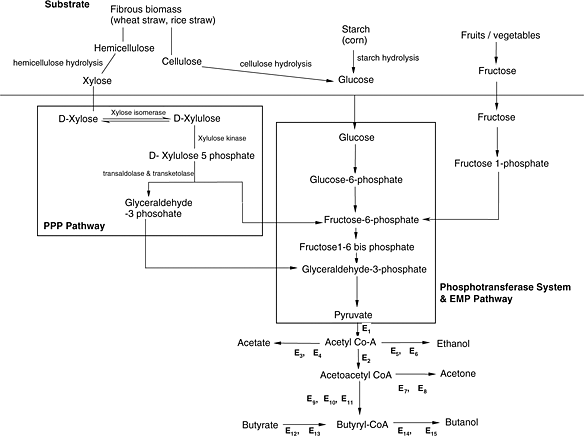
\includegraphics[width=\textwidth]{butanol-production}
    \end{center}
    \begin{textblock*}{50mm}(5mm,65mm)
        {\tiny Reproduced from A. Ranjan and V. S. Moholkar, Int. J. Energy Res., 36 (2012) 277--323}
    \end{textblock*}
\end{frame}

\begin{frame}{We can do engineering research on how the fuels will behave}
    \begin{itemize}
        \item We need to know the physical properties
        \begin{itemize}
            \item Density
            \item Viscosity
            \item \ldots
        \end{itemize}
        \item We need to know the \alert<2->{combustion properties}
        \begin{itemize}
            \item Heat of combustion
            \item Propensity to generate pollutants
            \item Reactivity
            \item \ldots
        \end{itemize}
    \end{itemize}
\end{frame}

\begin{frame}{We need both solutions to make substantial progress}
    \begin{itemize}
        \item Neither solution will be able to mitigate all of the negative impacts of combustion by itself
        \item Selecting the “best” alternative fuel requires knowledge of the “best” engine, which depends on which alternative fuel is selected…
        \item Computer-aided design and modeling can be employed to make new engines fuel-flexible \alert{if we have good models}
        \item Models must be validated with experimental data acquired under engine-relevant conditions
    \end{itemize}
\end{frame}

\begin{frame}{Combustion models are hierarchical}
    \only<1>{
    \begin{columns}[b]
        \column{0.65\textwidth}
            \begin{itemize}
                \item In this, ``combustion models'' = ``kinetic models'' = ``reaction mechanisms''
                \item Combustion chemistry is important! Studied since at least the advent of IC engines to understand knock; later for emissions and pollutants.
                \item Need to ensure that the models for small molecules are thoroughly validated when including them in models for large molecules
                \item A number of research efforts (past and present) have focused on this goal
            \end{itemize}
        \column{0.35\textwidth}
            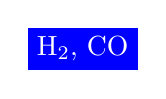
\begin{tikzpicture}
                \node[fill=blue,text=white,rectangle] at (0,0) {H$_2$, CO};
            \end{tikzpicture}
    \end{columns}
    }
    \only<2>{
    \begin{columns}[b]
        \column{0.65\textwidth}
            \begin{itemize}
                \item Model validation for larger molecule combustion must proceed in parallel to the small molecule chemistry because the models are needed now!
                \item Validation data for alcoholic alternative fuels has focused on the isomers of butanol (C4 alcohols) and i-pentanol (C5 alcohol)
            \end{itemize}
    \end{columns}
    }
    \only<3>{
    \begin{columns}[b]
        \column{0.65\textwidth}
            \begin{itemize}
                \item Models can predict the combustion of alcohols well for a variety conditions
                \item Models fail to predict certain engine relevant conditions, such as ignition delay dependence on [O2]
            \end{itemize}
    \end{columns}
    }
    \only<4>{
    \begin{columns}[b]
        \column{0.65\textwidth}
            \begin{itemize}
                \item Models of real transportation fuels are difficult to construct and use due to the chemical complexity of the fuels
                \item Surrogate models use a limited number of components to represent the chemical and physical properties of the real fuel
                \item Models need to be developed and validated for the neat components as well as for their blends
            \end{itemize}
    \end{columns}
    }
\end{frame}

\begin{frame}{Summary}
    \begin{itemize}
        \item We need a better understanding of the combustion properties of fuels we use now, fuels for the medium-term, and fuels for the long-term especially under engine-relevant conditions
        \item Using this understanding, we need to develop models that can predict the combustion behavior of new fuels in new engines
        \item My dissertation did x y z to advance these causes
    \end{itemize}
\end{frame}

\begin{frame}{Why Bio-Alcohols?}
\end{frame}

\begin{frame}{Why MCH?}
What are surrogates? (Has been touched on briefly previously)
\end{frame}

\section{Experimental Apparatuses}

\begin{frame}{Rapid Compression Machine}
    \only<+>{
    \begin{center}
        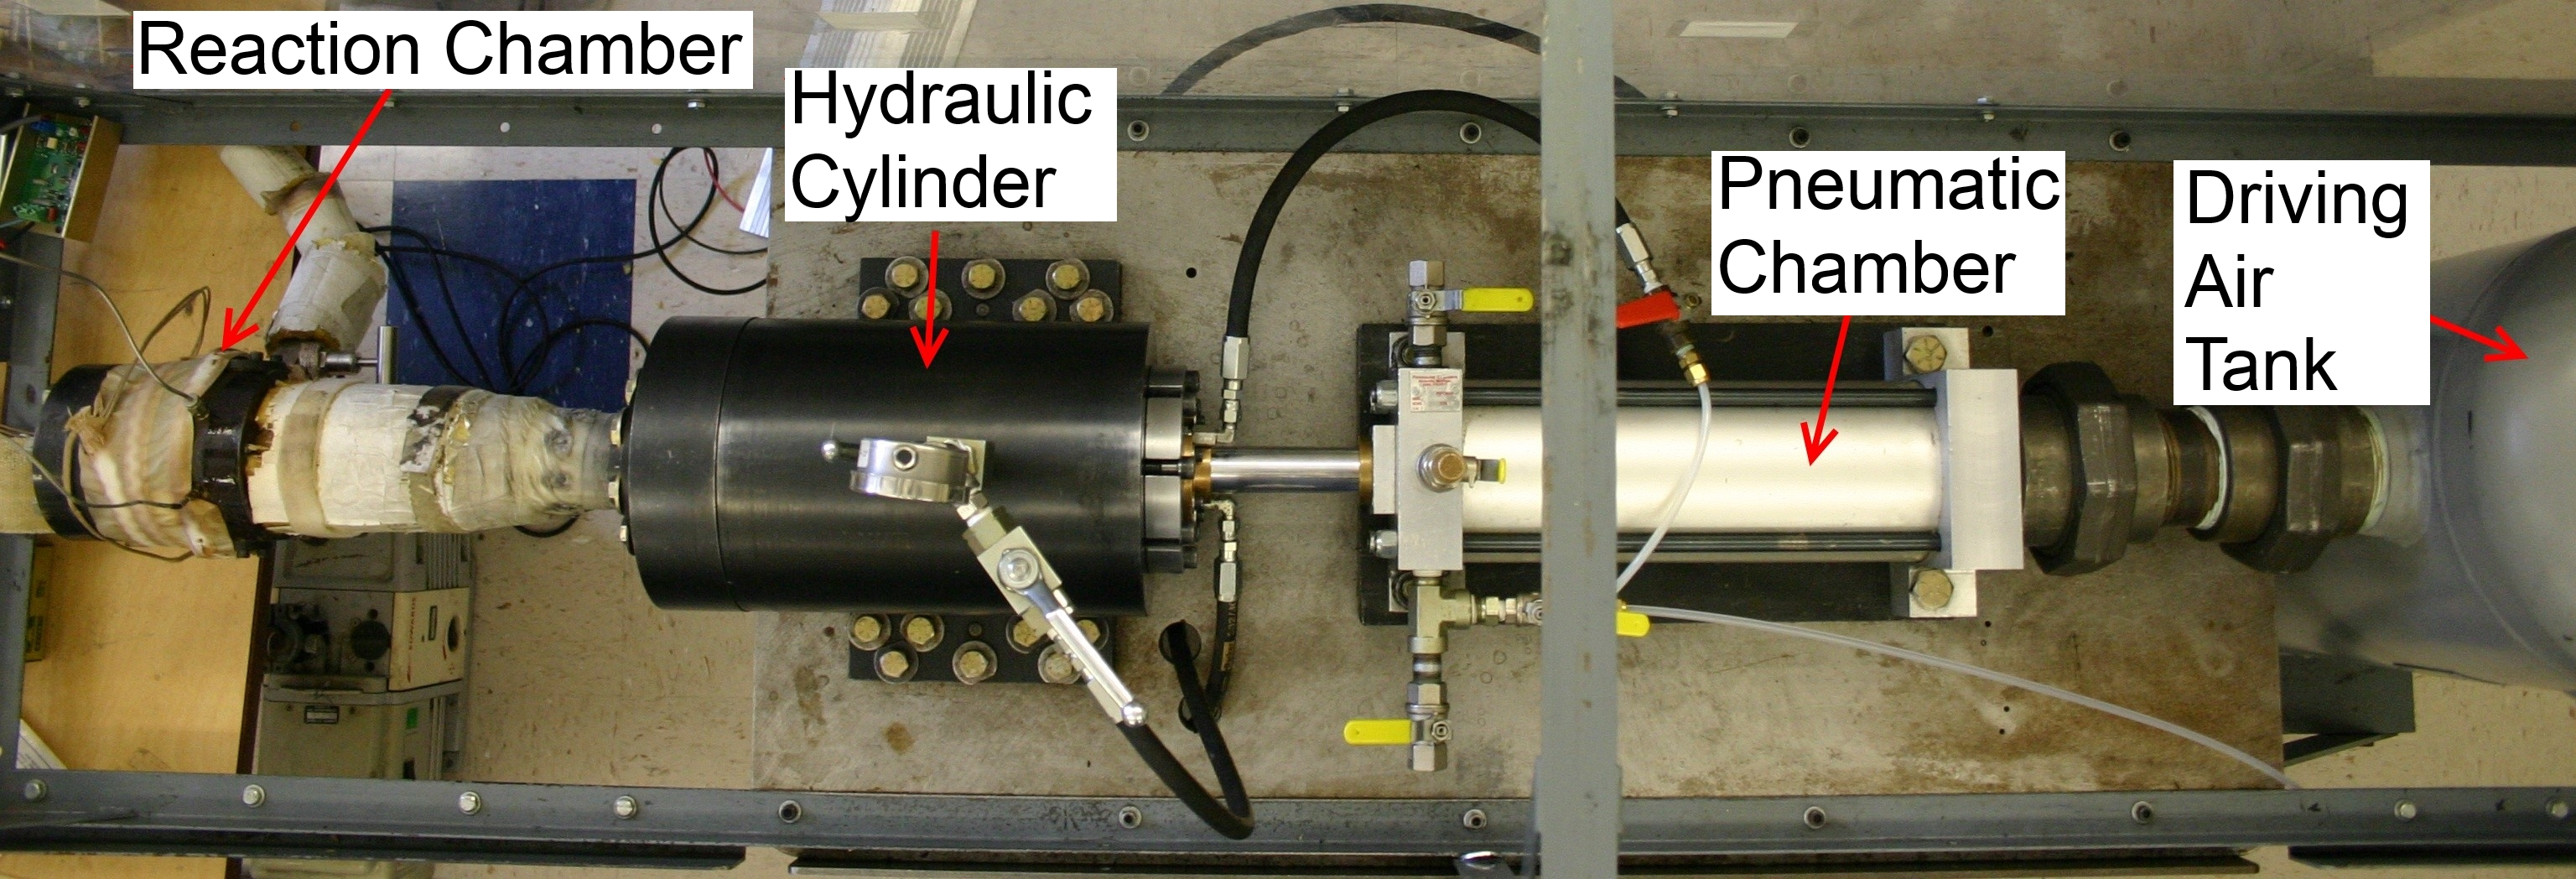
\includegraphics[width=\textwidth]{rcm-photo}
    \end{center}
    }
    \only<+>{
    \begin{center}
        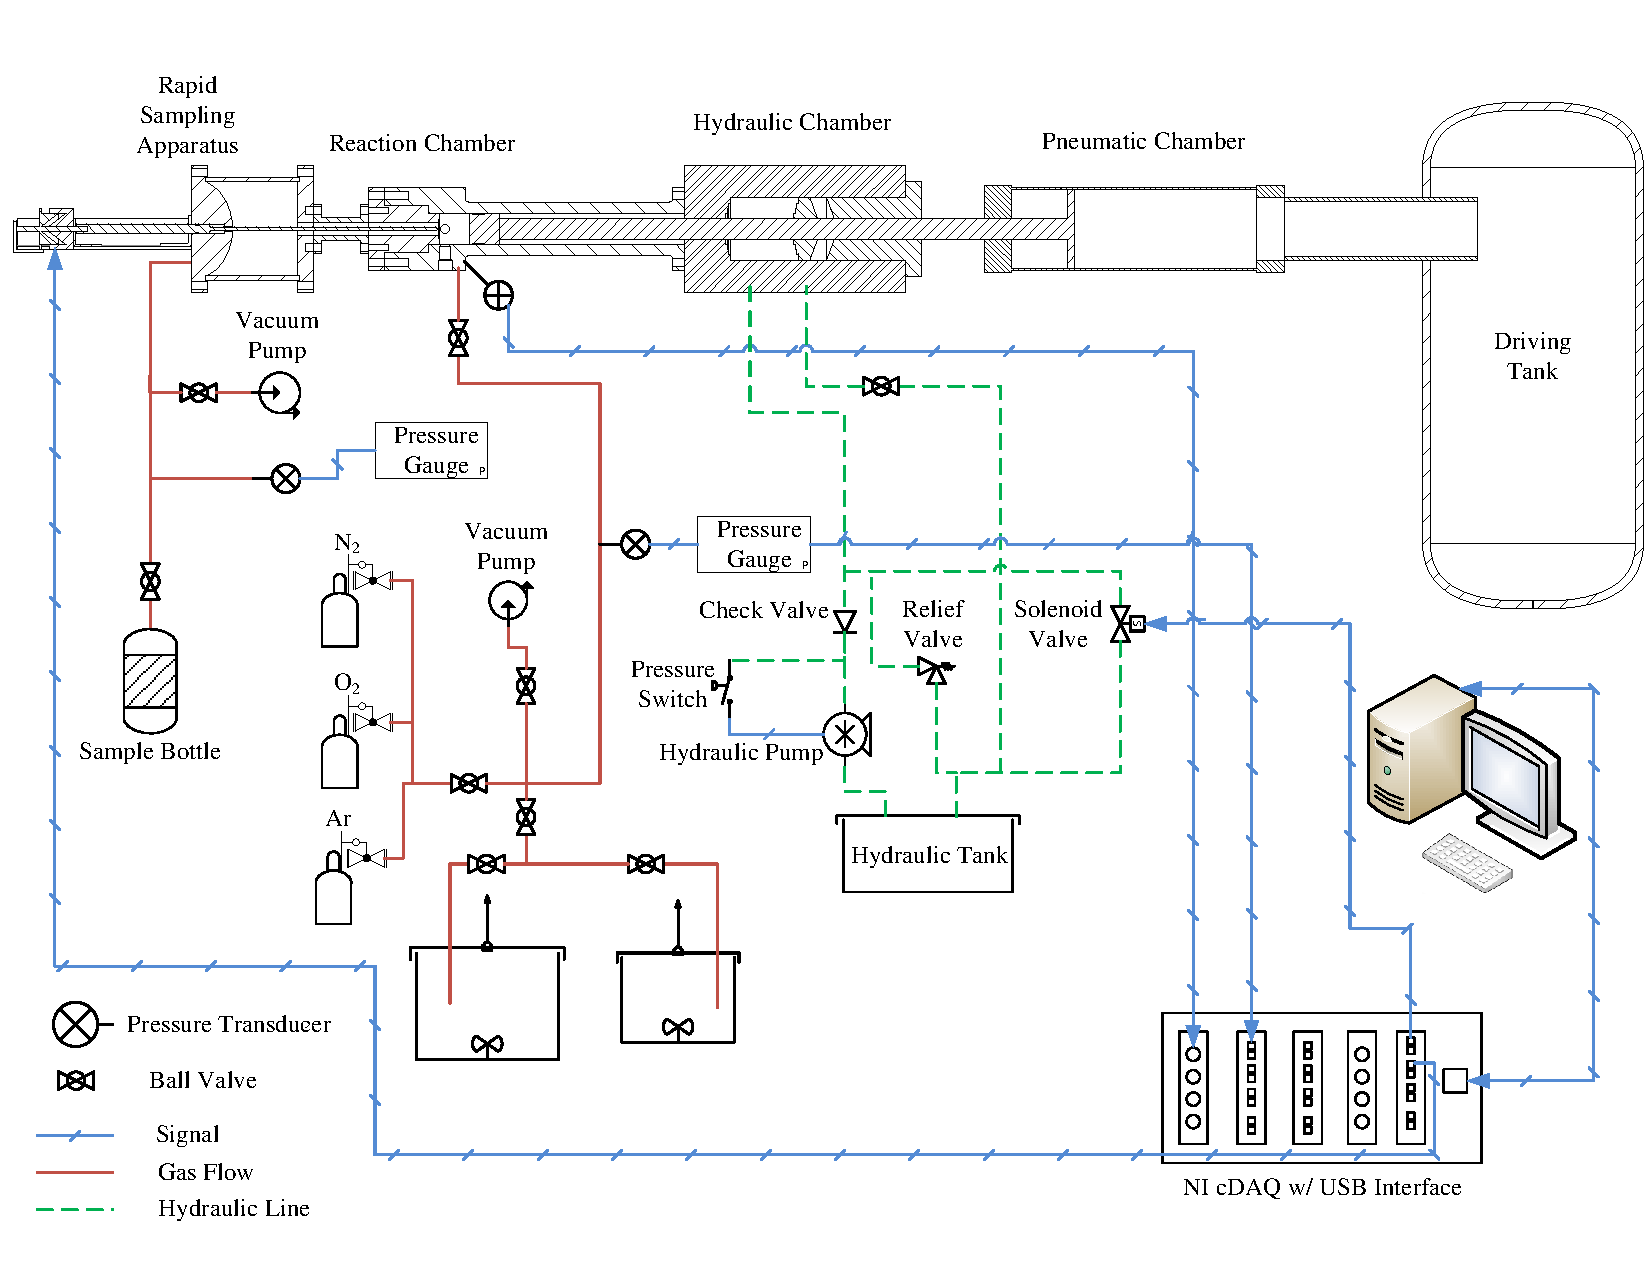
\includegraphics[width=\textwidth,height=0.95\textheight,keepaspectratio]{rcm-schematic}
    \end{center}
    }
\end{frame}

\begin{frame}{Rapid Sampling Apparatus}
    \begin{columns}
        \column{0.6\textwidth}
        \begin{minipage}[c][0.6\textheight][c]{\linewidth}
            \begin{itemize}
                \item Sampling apparatuses have been used since the 1920's to study combustion chemistry
                \item<2-> In the 1960's, the first sampling apparatus was adapted for an RCM
                \item<3-> Mittal developed a similar system for the present RCM based on deactivating an electromagnet
                \item<4-> I have modified the design of Mittal to incorporate a solenoid instead of the electromagnet
            \end{itemize}
        \end{minipage}
        \only<+>{
        \column{0.4\textwidth}
            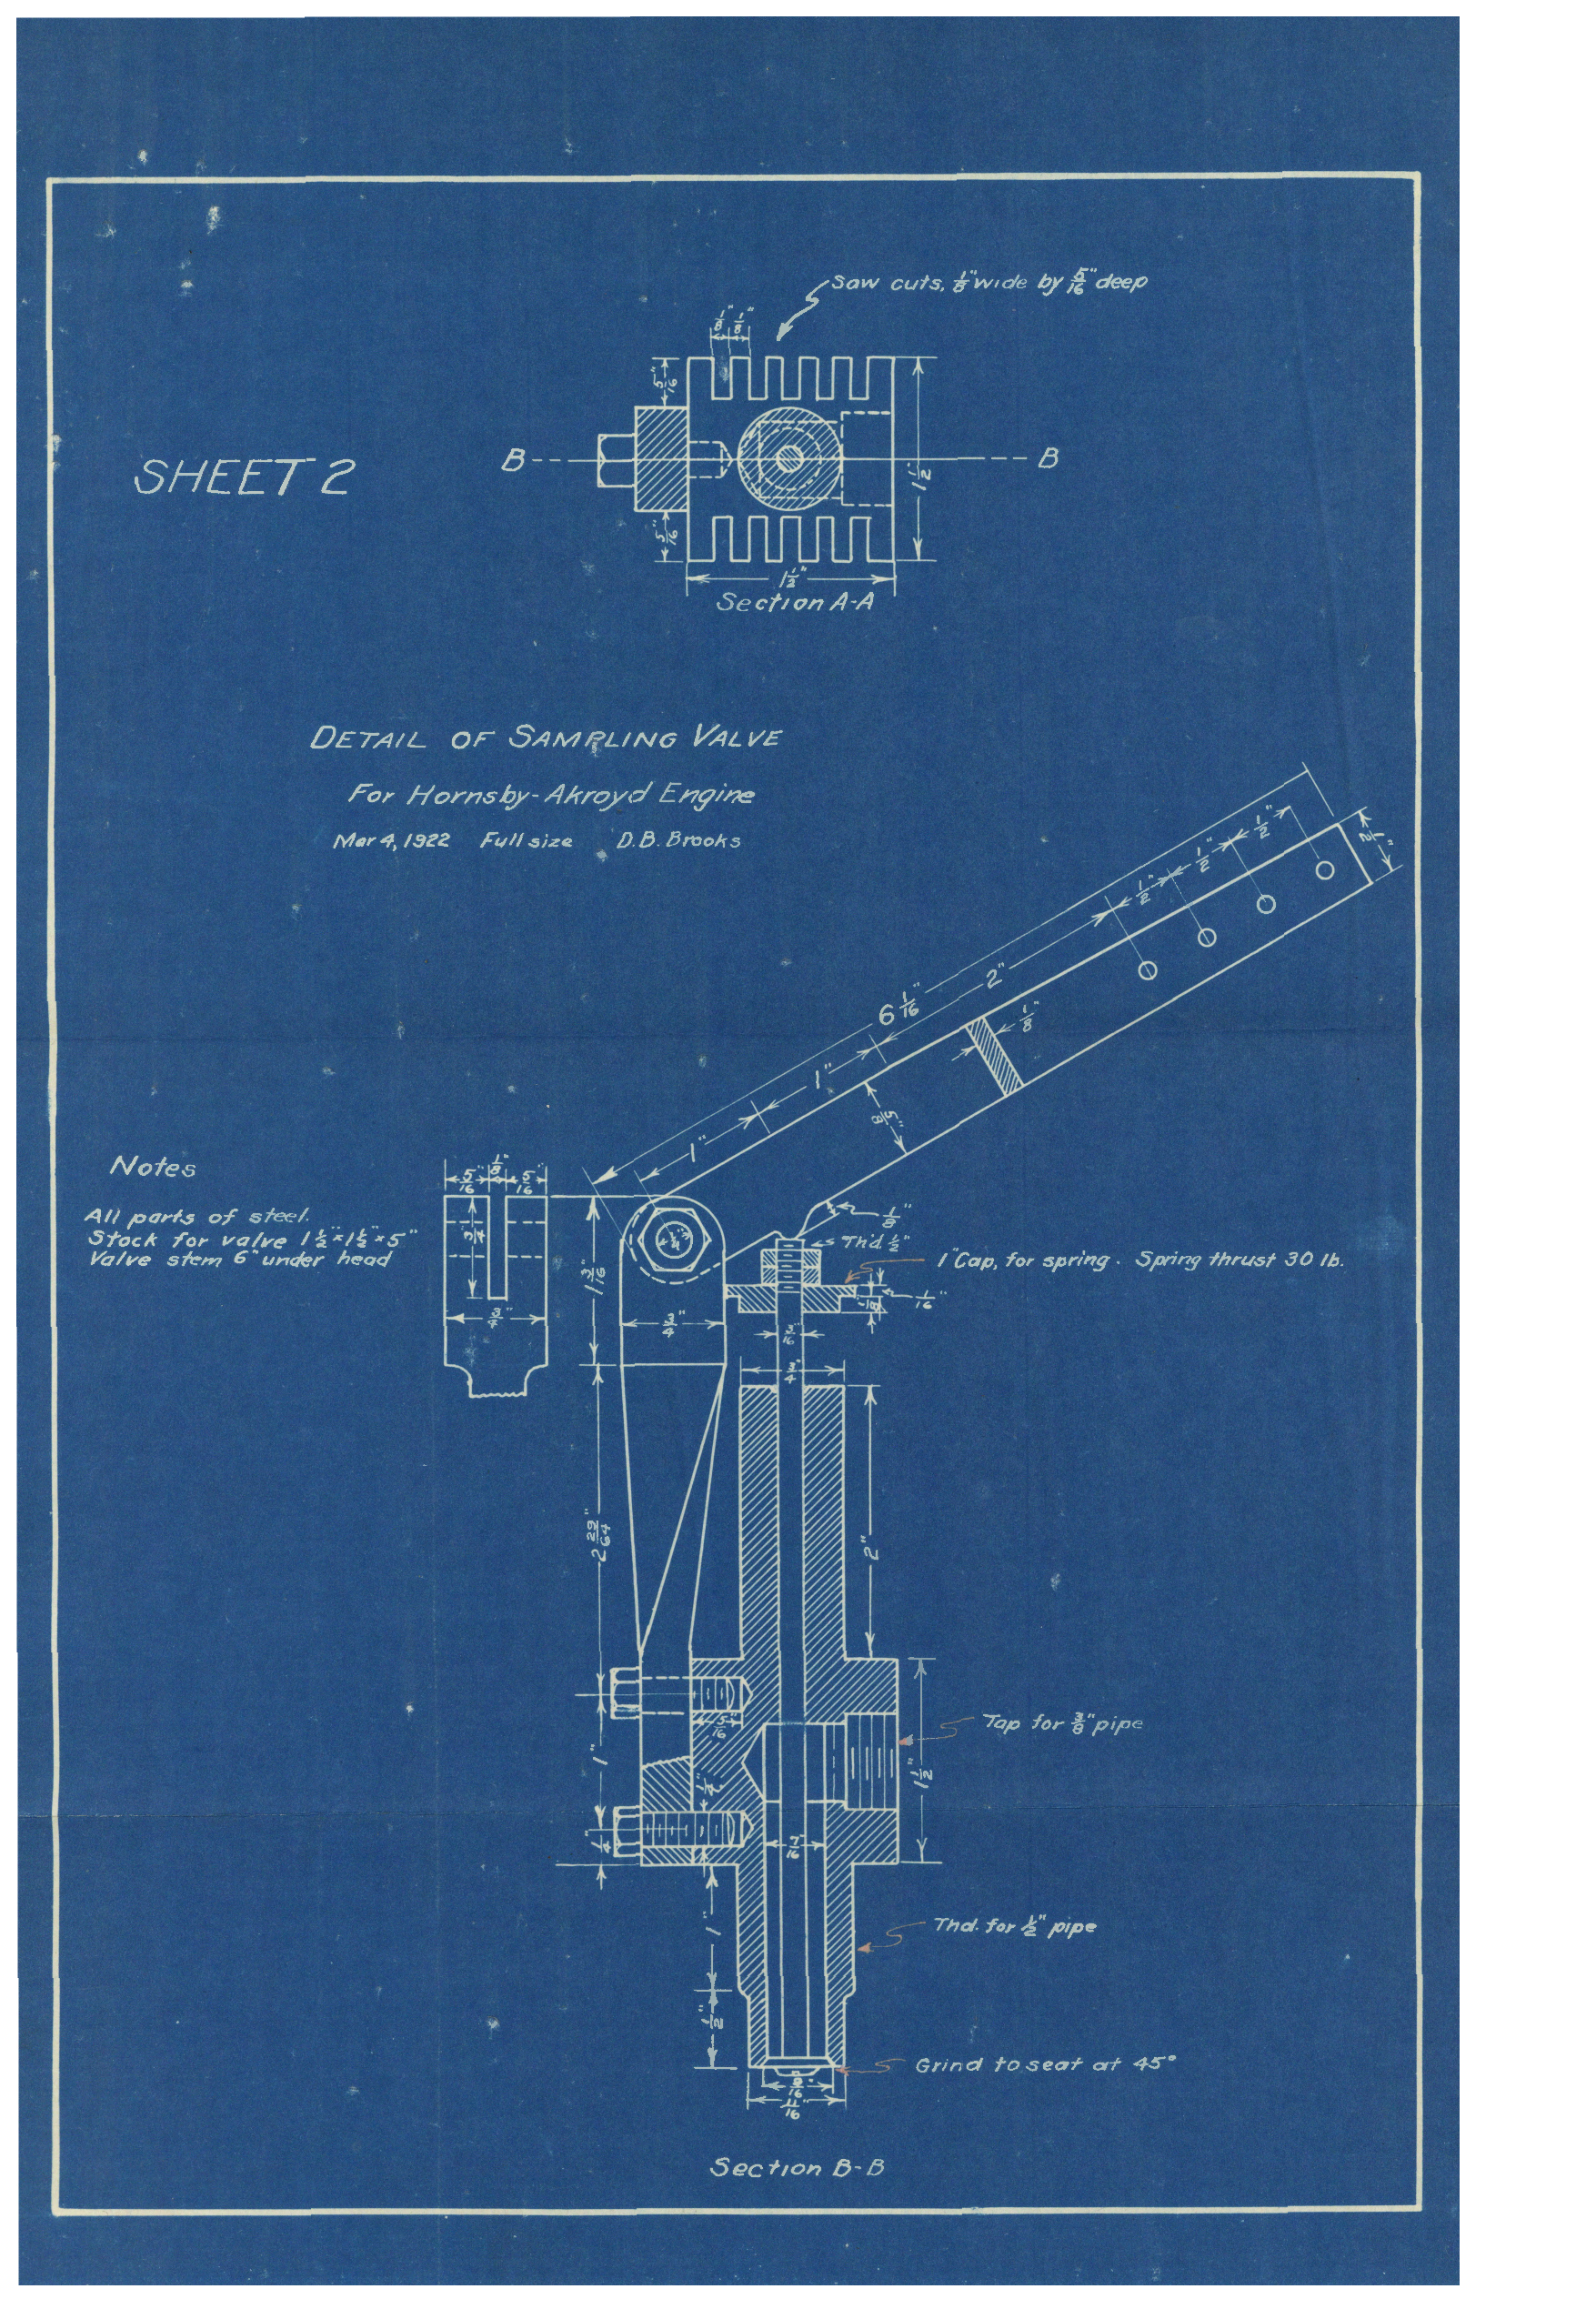
\includegraphics[width=\textwidth]{brooks}
        }
        \only<+>{
        \column{0.4\textwidth}
            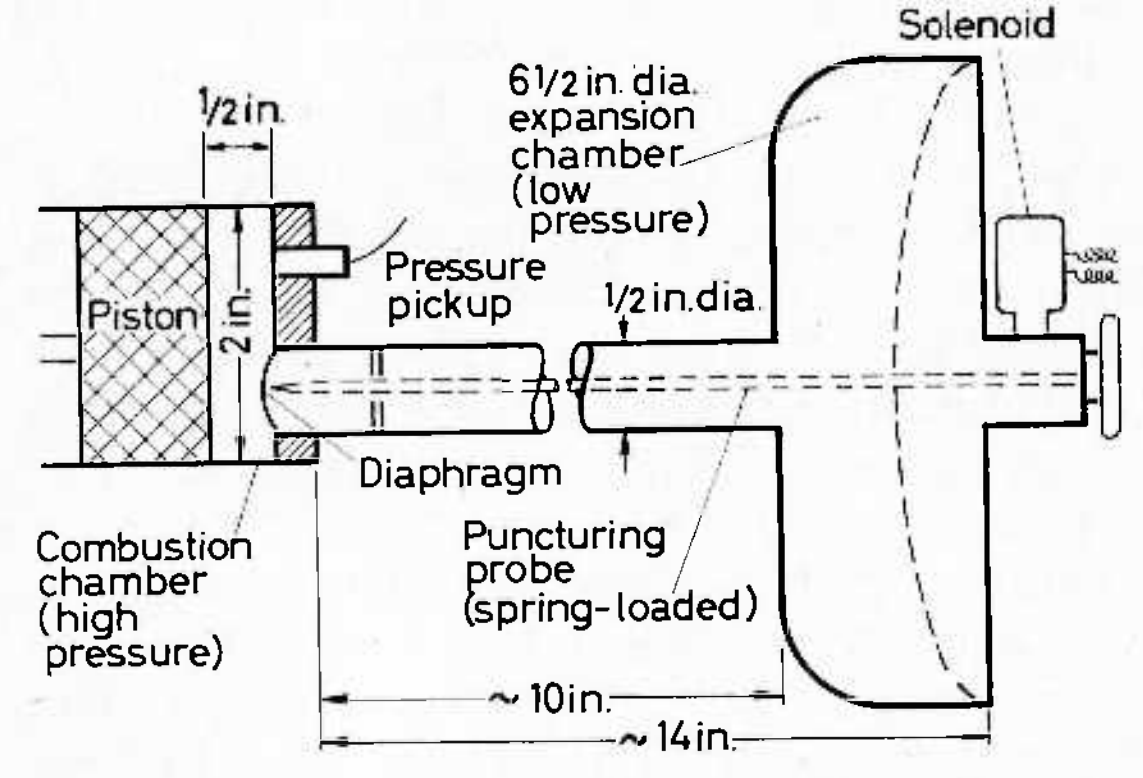
\includegraphics[width=\textwidth]{roblee-sampling}
        }
    \end{columns}
\end{frame}

\begin{frame}{Gas Chromatograph/Mass Spectrometer}
    \begin{itemize}
        \item Standard piece of chemistry lab equipment, commercially supplied (Shimadzu)
        \item Separates, identifies, and quantifies chemical species
    \end{itemize}
\end{frame}

\end{document}
